\subsection{Osservazione qualitativa degli andamenti (si puo cambiare)}

\begin{figure}[h]
    \centering
    \includegraphics[width=1\textwidth]{../figs/tensione-tempo.pdf}
    \caption{ampiezze}\label{fig:tensione-tempo}
\end{figure}

Una volta scelti i valori dei componenti da utilizzare per l’esperienza di laboratorio e calcolato il valore atteso della
frequenza di risonanza che, come citato precedentemente, corrisponde a...., è stato analizzato dal punto di vista qualitativo il comportamento del circuito per verificare che fosse in accordo con quanto previsto e descritto nella sezione “Introduzione”.
Come si può osservare nella figura 2., andando a studiare frequenze costanti della tensione in ingresso, prossime al valore di risonanza, l’andamento della tensione sulla resistenza è risultato essere in fase con quello indotto sul generatore, come ci si aspettava dal punto di vista teorico.
L’anomalia riscontrata sul primo periodo delle acquisizioni effettuate a tensioni costanti verrà analizzata e descritta nella sezione “Appendice” di seguito.

\subsection{Analisi delle ampiezze}

Gli andamenti della tensione ai capi di ciascun componente e del circuito stesso, ottenuti da calcoli svolti dal programma di acquisizione dati Labview al variare della frequenza, sono mostrati nella figura 3.
L’incertezza associata alle tensione è stata ottenuta come la deviazione standard delle misure associate all’ampiezza della tensione agli estremi, che sono perciò posti costanti, ottenendo quindi come valore …..
Qui di seguito sono mostrate le funzioni che descrivono l’andamento del modulo dell’ampiezza ai capi di ciascun componente e il procedimento adottato per ricarvarle viene analizzato con più attenzione nella sezione “Appendice”.

\[
    V_R = \frac{R_rV_0}{\sqrt{{(R_r+R)}^2+{ \left(\omega L - \frac{1}{\omega C}\right)}^2}}
\]
\[
    V_L = \frac{\omega L V_0}{\sqrt{R^2+{ \left(\omega L - \frac{1}{\omega C}\right)}^2}}
\]
\[
    V_C = \frac{\frac{V_0}{\omega C}}{\sqrt{R^2+{ \left(\omega L - \frac{1}{\omega C}\right)}^2}}
\]

\begin{figure}[h]
    \centering
    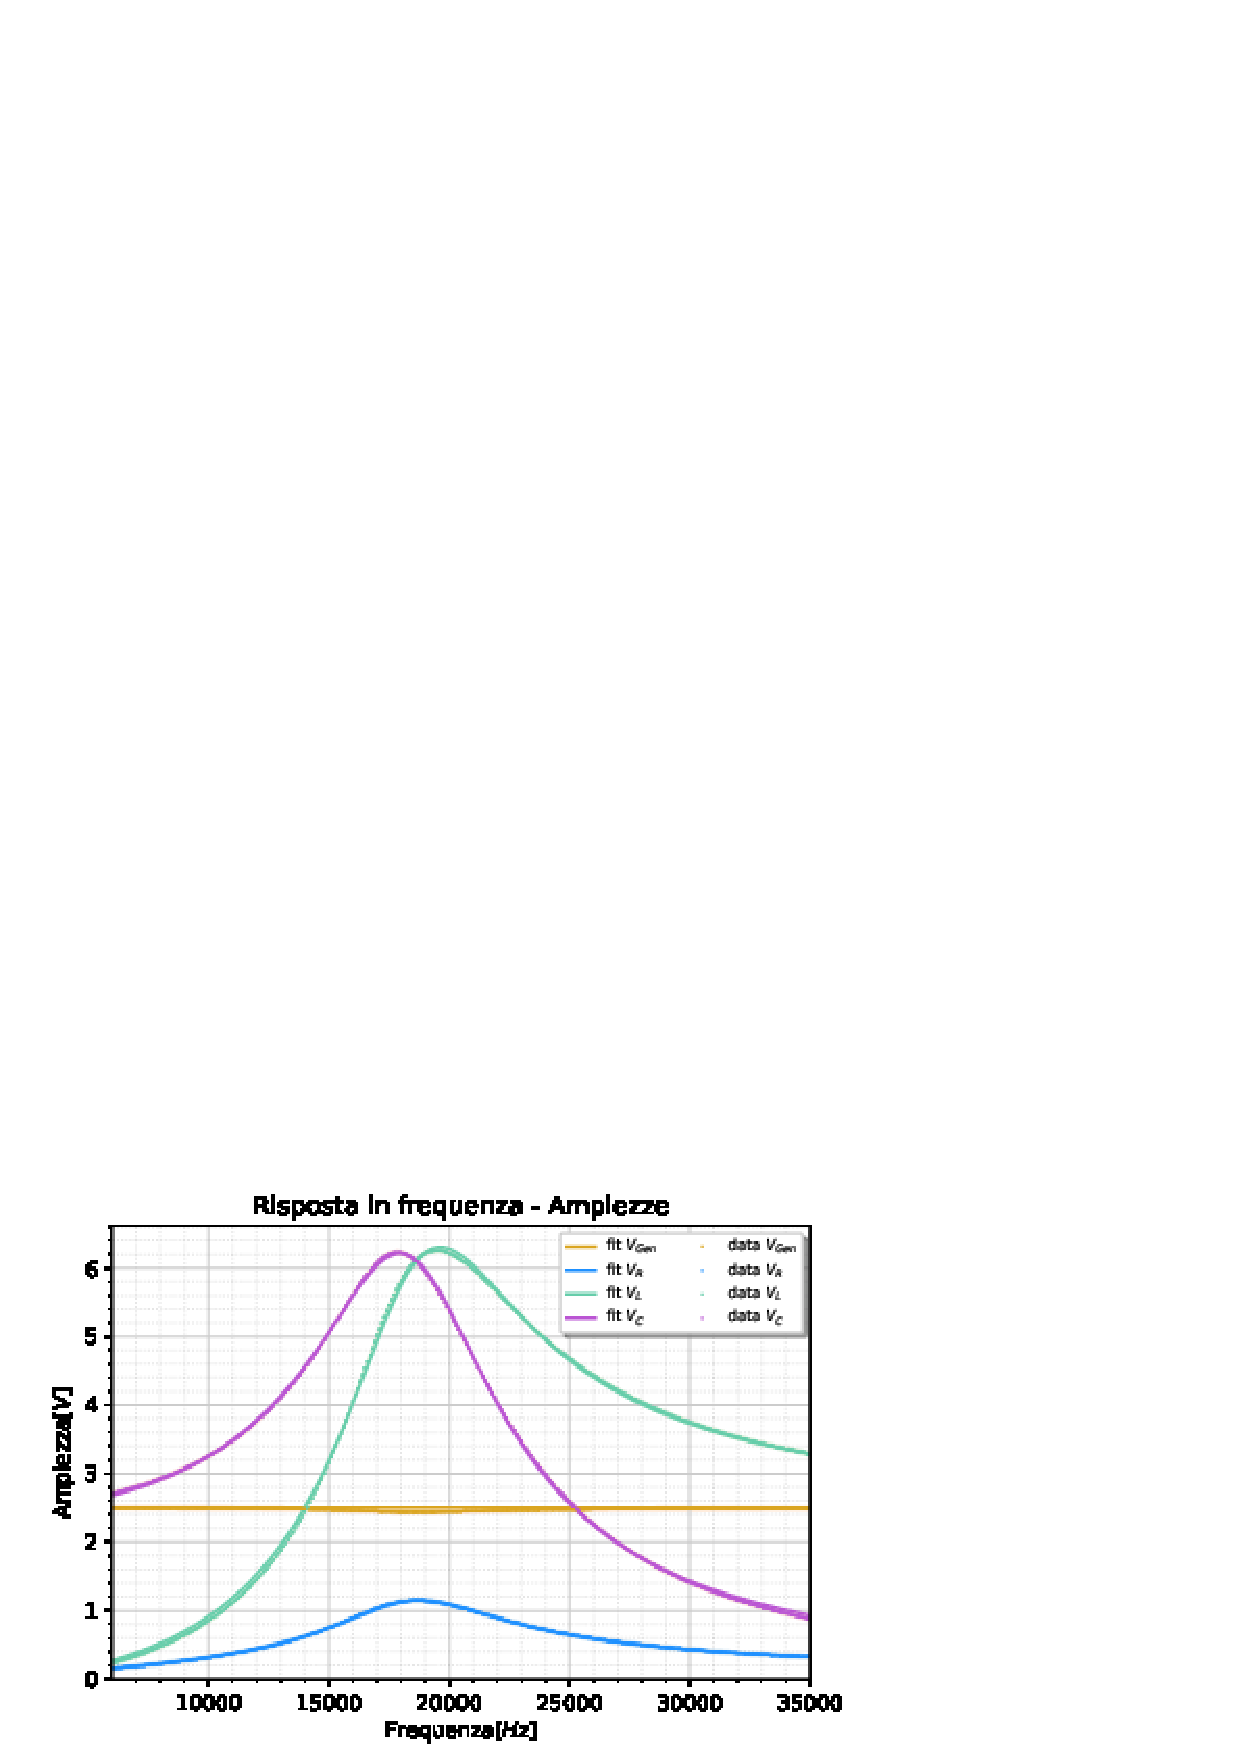
\includegraphics[width=1\textwidth]{../figs/Risposta-in-frequenza-ampiezze.pdf}
    \caption{ampiezze}\label{fig:ampiezzeRLC}
\end{figure}


\begin{figure}[h]
    \centering
    \includegraphics[width=.9\textwidth]{../figs/Risposta-in-frequenza-ampiezza-resistenza.pdf}
    \caption{cambia grafico con nuovi valori fit parametri}\label{fig:ampiezzeR}
\end{figure}




Rr rappresenta la resistenza escludendo però quelle interne a generatore e induttanza, mentre omega indica la pulsazione della tensione applicata.
Andando ad analizzare l’andamento della tensione ai capi di ciascun componente e del circuito stesso, si può notare che l’ampiezza della tensione indotta nel circuito prensenta un picco per valori della frequenza prossimi a quella di risonanza per poi presentare valori più bassi via via che ci si allontana da questa condizione.
Questo effetto è dovuto alla resistenza interna del generatore che provoca una caduta di potenziale proporzionale alla corrente che attraversa il circuito, il cui valore in modulo è massimo proprio in corrispondenza della frequenza di risonanza.
I valori del chi quadro che sono stati ottenuti dai fit sui tre componenti sono...
Si è poi optato di calcolare il valore della frequenza di risonanza con i parametri ottenuti dal fit mediante l’utilizzo dell’equazione 1.
Andando a considerare il fit associato alla resistenza, mostrato in figura 4, i parametri utilizzati sono L=…. e C =….., in questo modo si è controllato se il valore della frequenza di risonanza atteso e calcolato a livello teorico potesse coincidere con quello ottenuto, che è risultato essere di...., dove le incertezze sono state propagate in quadratura.
Un modo alternativo per determinare il valore della frequenza di risonanza è studiare il punto di massimo del grafico relativo all’ampiezza della tensione ai capi della resistenza utilizzata per l’esperienza di laboratorio, ma, non essendo sicuri dell’incertezza sulla misura della tensione, si è deciso di stimare un range di valori.
Preso l’estremo inferiore della barra di errore relativa al punto di massimo estratto dal fit, si sono poi cercati i punti in cui l’estremo superiore della barra di errore corrispondesse a tale valore massimo. In questo modo, però, si è sovrastimata l’incertezza relativa alla frequenza di risonanza, calcolandola come il valore medio di questi due estremi.
Si è ottenuto in questo modo un valore della frequenza di risonanza pari a....
Il valore centrale dell’intervallo scelto è consistente con quanto ottenuto utilizzando i parametri del fit, ma a causa della sovrastima dell’incertezza il risultato può essere considerato poco rilevante.

Parlare eventualmente del valore più alto della resistenza.







\subsection{Analisi delle fasi}

Le funzioni che descrivono gli andamenti attesi delle fasi sono le seguenti:
 \[
     \phi_R = \arctan{\frac{1 - \omega^2 L C}{R \omega C}}
 \]
\[
    \phi_L = \arctan{\frac{1 - \omega^2 L C}{R \omega C}} + \frac{\pi}{2}
\]
 \[
     \phi_C = \arctan{\frac{1 - \omega^2 L C}{R \omega C}} - \frac{\pi}{2}
 \]

\begin{figure}[h]
    \centering
    \includegraphics[width=.9\textwidth]{../figs/Risposta-in-frequenza-fasi.pdf}
    \caption{fasi }\label{fig:fasi}
\end{figure}

Si è poi pensato di estrarre il valore corrispondente a una condizione di fase nulla tra la curva associata alla resistenza e quella del generatore, che risulta essere di..., andando a ripetere lo stesso procedimento analizzando questa volta la curva associata all’induttanza ma, considerando uno sfasamento di 90 gradi, si è ottenuto una misura della frequenza pari a... anch’essa vicina al valore atteso, anche se risulta essere sovrastimata.

